% The BLAKE3 compression function [BLAKE3, §2.2]: the state is the chaining value h, four IV
% words, the counter t = (t0, t1), the block length b and the flags d. Seven rounds of the
% BLAKE2s round follow, with the message words permuted between rounds; the output is
% (v_lo xor v_hi, v_hi xor h), whose first half is the next chaining value.
% Original drawing for the Hash library.
\documentclass[tikz,border=6pt]{standalone}
\usepackage[T1]{fontenc}
\usepackage{lmodern}
% Shared style for the Hash diagrams.
% Palette: Okabe–Ito (colour-blind safe). Every diagram is drawn on an opaque white card so it
% stays legible on dark page themes.
\usetikzlibrary{arrows.meta,positioning,calc,fit,backgrounds}
\definecolor{hsblue}{HTML}{0072B2}
\definecolor{hsorange}{HTML}{E69F00}
\definecolor{hsgreen}{HTML}{009E73}
\definecolor{hsvermilion}{HTML}{D55E00}
\definecolor{hspurple}{HTML}{CC79A7}
\definecolor{hsink}{HTML}{1F2933}
\tikzset{
  >={Stealth[length=2.2mm]},
  every node/.style={font=\sffamily\small, text=hsink},
  wire/.style={draw=hsink, line width=0.6pt, ->},
  reg/.style={draw=hsink, line width=0.6pt, fill=hsblue!12, minimum width=9mm, minimum height=7mm},
  fn/.style={draw=hsink, line width=0.6pt, fill=hsorange!25, rounded corners=2pt, minimum width=10mm, minimum height=6mm},
  input/.style={draw=hsink, line width=0.6pt, fill=hsgreen!20, minimum width=9mm, minimum height=6mm},
  add/.style={circle, draw=hsink, line width=0.6pt, fill=white, inner sep=0pt, minimum size=5mm, font=\sffamily\bfseries},
  card/.style={fill=white, rounded corners=4pt},
}

\begin{document}
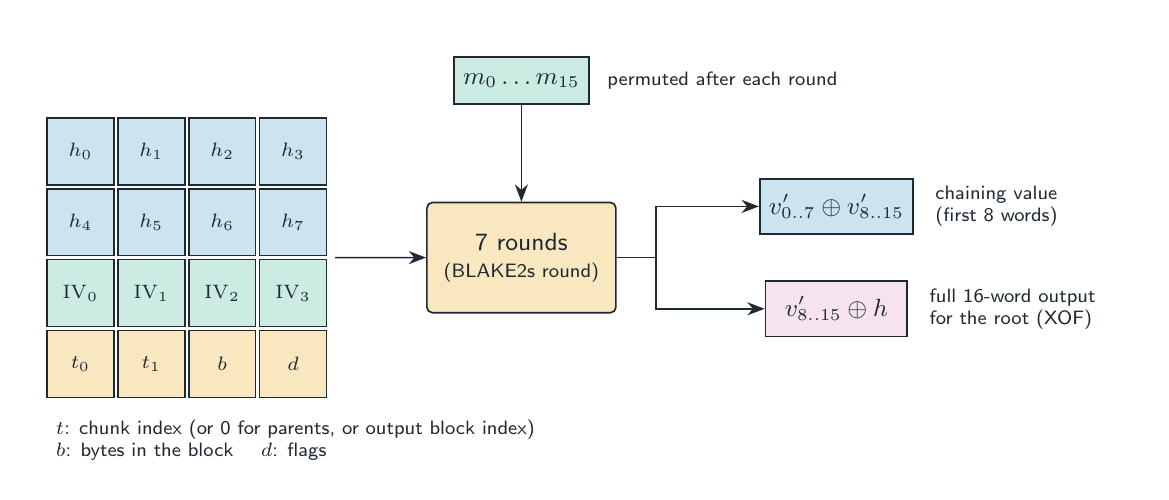
\begin{tikzpicture}[cell/.style={draw=hsink, line width=0.6pt, minimum size=8.5mm, inner sep=0pt,
    font=\sffamily\scriptsize}]
  \def\s{0.9}
  \foreach \r in {0,...,3} \foreach \c in {0,...,3} {
    \pgfmathtruncatemacro{\i}{4*\r+\c}
    \ifnum\r<2 \def\col{hsblue!20}\def\lbl{$h_{\i}$}
    \else\ifnum\r=2 \def\col{hsgreen!20}\def\lbl{$\mathrm{IV}_{\c}$}
    \else \def\col{hsorange!25}\ifcase\c\def\lbl{$t_0$}\or\def\lbl{$t_1$}\or\def\lbl{$b$}\or\def\lbl{$d$}\fi\fi\fi
    \node[cell, fill=\col] (v\i) at (\c*\s, -\r*\s) {\lbl};
  }
  \node[fn, minimum width=24mm, minimum height=14mm, align=center, font=\sffamily\small] (E)
    at (5.6, -1.35) {7 rounds\\[-1pt]{\scriptsize (BLAKE2s round)}};
  \draw[wire] ($(v3.east)!0.5!(v15.east)+(0.1,0)$) -- (E.west);
  \node[input, minimum width=14mm] (m) at (5.6, 0.9) {$m_0 \ldots m_{15}$};
  \draw[wire] (m) -- (E);
  \node[font=\sffamily\scriptsize, anchor=west] at ($(m.east)+(0.1,0)$) {permuted after each round};
  \node[reg, minimum width=18mm, fill=hsblue!20] (lo) at (9.6, -0.7) {$v'_{0..7} \oplus v'_{8..15}$};
  \node[reg, minimum width=18mm, fill=hspurple!20] (hi) at (9.6, -2.0) {$v'_{8..15} \oplus h$};
  \draw[wire] (E.east) -- ++(0.5,0) |- (lo.west);
  \draw[wire] (E.east) -- ++(0.5,0) |- (hi.west);
  \node[font=\sffamily\scriptsize, anchor=west, align=left] at ($(lo.east)+(0.15,0)$)
    {chaining value\\(first 8 words)};
  \node[font=\sffamily\scriptsize, anchor=west, align=left] at ($(hi.east)+(0.15,0)$)
    {full 16-word output\\for the root (XOF)};
  \node[font=\sffamily\scriptsize, anchor=north west, align=left] at ($(v12.south west)+(0,-0.15)$)
    {$t$: chunk index (or 0 for parents, or output block index)\\
     $b$: bytes in the block \quad $d$: flags};
  \begin{scope}[on background layer]
    \coordinate (e1) at (-0.6,-4.0);
    \coordinate (e2) at (13.4,1.5);
    \node[card, fit=(e1)(e2), inner sep=2pt] {};
  \end{scope}
\end{tikzpicture}
\end{document}
